\chapter{Software Installation and Package Management}
\label{chap:software-installation}

\begin{quote}
{\em There is no neat distinction between operating system software
and the software that runs on top of it.} --
Jim Allchin\index[names]{Allchin, Jim}
\end{quote}

% XXX better graphic
\begin{figure}[hb]
	\raggedleft
	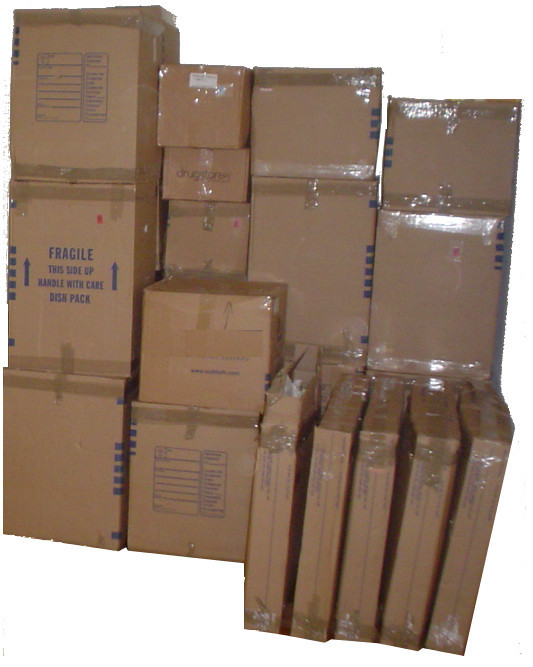
\includegraphics[width=.25\textwidth]{05/pics/many-boxes}
\end{figure}

\section{Introduction}
\label{software-installation:introduction}

%\begin{figure}[b]
%	\captionsetup{justification=justified,singlelinecheck=false}
%	\caption[Moving Boxes]{As anybody preparing a move knows,
%		handling all your boxes frequently ends in organized
%		chaos at best.  Managing software packages is not very	
%		different.
%		\label{fig:many-boxes}}
%\end{figure}


Having covered the details of file systems and storage
devices in the previous chapter, we can now focus on
installing an operating system and adding software
according to the intended purpose of the system.  Most
people never have to actually perform an OS
installation, but System Administrators are not most
people.  We routinely set up new systems, create new
services, and need to be able to fine-tune the
software from the very lowest layers, defining exactly
what software is installed, what drivers the kernel
needs to support, what modules it should load, and
what services should be started at boot time.

In addition, even within a single host, some subsystems
that control components on a lower layer than even the
OS kernel, such as a RAID controller or a Fibre
Channel \gls{hba}, are driven by their own
firmware\index{firmware}, accessed by the OS via its
kernel drivers and exposed to the administrative users
via additional software tools.  All of these types of
software have specific requirements, yet all of them
also have in common the general mechanisms to install,
update, maintain and remove the software.

In this chapter we will discuss in some detail the
general principles underlying all software
installations, beginning with a distinction of the
different types of software we commonly encounter,
most notably the two main categories of OS components
and {\em add-on} or {\em third-party} software.  We
will look at how an operating system is installed on a
server and what installation mechanisms are commonly
used.  Since different operating systems install
different components into different locations, we will
also take a close look at the file system layout and
explain some of the reasons behind the common
hierarchy found on most Unix systems.

Later in the chapter, we will cover concepts of
software package management that allow a system
administrator to not only add or remove software with
ease, but to help maintain software runtime
dependencies and provide a consistent way to upgrade
software when needed.  Unfortunately, software package
management is still not a solved problem: managing
software updates and security patches brings with it a
surprising number of complex problems, in part due to
competing solutions in this problem domain.  All of
this does not even touch upon the evolution of how
applications are bundled in the context of virtual
machines, virtual appliances, and software
containers\index{containers}. \\

Every system administrator has a preferred operating
system, and this preference is often the result of
years of experience and familiarity not only with the
kernel and libraries that make up the OS, but
frequently also due to the package management system
in use on the host.  Just how, exactly, a package
manager maintains software dependencies, what kinds of
assumptions it makes about the system it is running
on, its purpose, and its many uses all reflect deeply
on the OS development philosophy.  The way software
updates are handled speaks volumes about both the
system as well as its administrators -- the better we
understand software installation concepts, the better
we will be at managing our systems.  Understanding all
this just a little bit better is, in a nutshell, what
this chapter is all about.

\section{Types of Software}
\label{software-installation:types}
\index{Software!Types of}

In its most general definition, ``software'' is just
another term for a program telling a computer to
perform a certain task.  Practically, however, there
are a number of different types of software.  In this
section, we will attempt to categorize these types,
even though the distinctions or differentiating
factors are far from clear-cut.

In the previous chapter, we have already identified a
specific component that happens to be implemented in
software: the file system.  Instinctively, we
categorize the file system as being in a lower layer
than certain applications, such as a web server for
example.  But the file system is only one component of
the operating system, which in turn comprises regular
application software (such as a text editor or a
compiler), software libraries used by many of these
applications (such as the resolver library, used to
turn hostnames into IP addresses), device
drivers\index{device driver} providing access to and
control of certain hardware components, and the most
central component of the OS itself, the
kernel\index{kernel}.

Looking at software from this perspective quickly
makes it clear that the term ``operating system''
itself requires some definition, as different
providers include different components under this
umbrella term.  Recall from our discussion of the Unix
history in Section \ref{unix:history:os} that the term
``Linux'', for example, may refer to the linux
kernel as well as any number of ``distributions'',
each bundling a variety of components to make up a
version of the GNU/Linux operating system.  But before
we attempt to tackle the question of what, exactly,
defines an operating system, let us take a step back
and attempt to better categorize software based on its
proximity to the hardware or the end user.

\subsection{Up and down the software stack}
\label{software-installation:boot-sequence}

One of the most common systems a system administrator
may be in charge of is probably a generic
HTTP\index{HTTP} server, offering a web service of
some sort.  Such a service nowadays consists of a
perhaps surprising number of components and software
dependencies running -- in our example here, anyway --
on virtual hardware within the AWS cloud service.
From a "top down" perspective, it might:

\begin{itemize}
	\item require an HTTP server -- the actual d\ae mon
		handling the network connections on
		port 80 and 443
	\item require e.g. PHP, Perl, Python, Ruby, or Java --
		entirely static pages are seldom found
		on the internet; instead, most web
		servers provide dynamic content via
		integration with other programming
		languages and modules
	\item which use generic library functions --
		the web server and the programming
		languages or frameworks are utilizing
		the standard libraries available on
		the system
	\item which make various system calls (see
		our discussion in Chapter \ref{unix:basics})
	\item which the kernel handles for the OS
	\item which is running in a virtual machine\index{virtual machine} --
		in the case of AWS, the OS our server is
		running on does not actually sit on
		top of the hardware itself
	\item which is running on top of a {\em
		hypervisor}\index{hypervisor} -- the
		host system managing the hardware for
		the different {\em guest} OS, such as
		for example the Xen
		hypervisor\index{Xen}
	\item which uses firmware to manage various
		hardware components
	\item which, finally, is running on some
		hardware in a data center somewhere
\end{itemize}

Going down this stack, we can already identify a number of
different interacting and overlapping categories of
software.  As such a Unix system boots up, it goes
through a number of phases, each of which handled by a
different type of software.  The typical boot sequence
begins at a very low level close to the hardware and
with each step adds another layer of abstraction,
bringing the system closer to interaction with the
user.

In order not to complicate things more than absolutely
necessary, we will skip over the layers involving the
hypervisor in the following.  Pretending that the OS
runs on actual, not virtual hardware, the boot process
might then include these steps:

\begin{figure}[t]
	\subfloat[American Megatrends POST]{\label{fig:software-installation:post}
				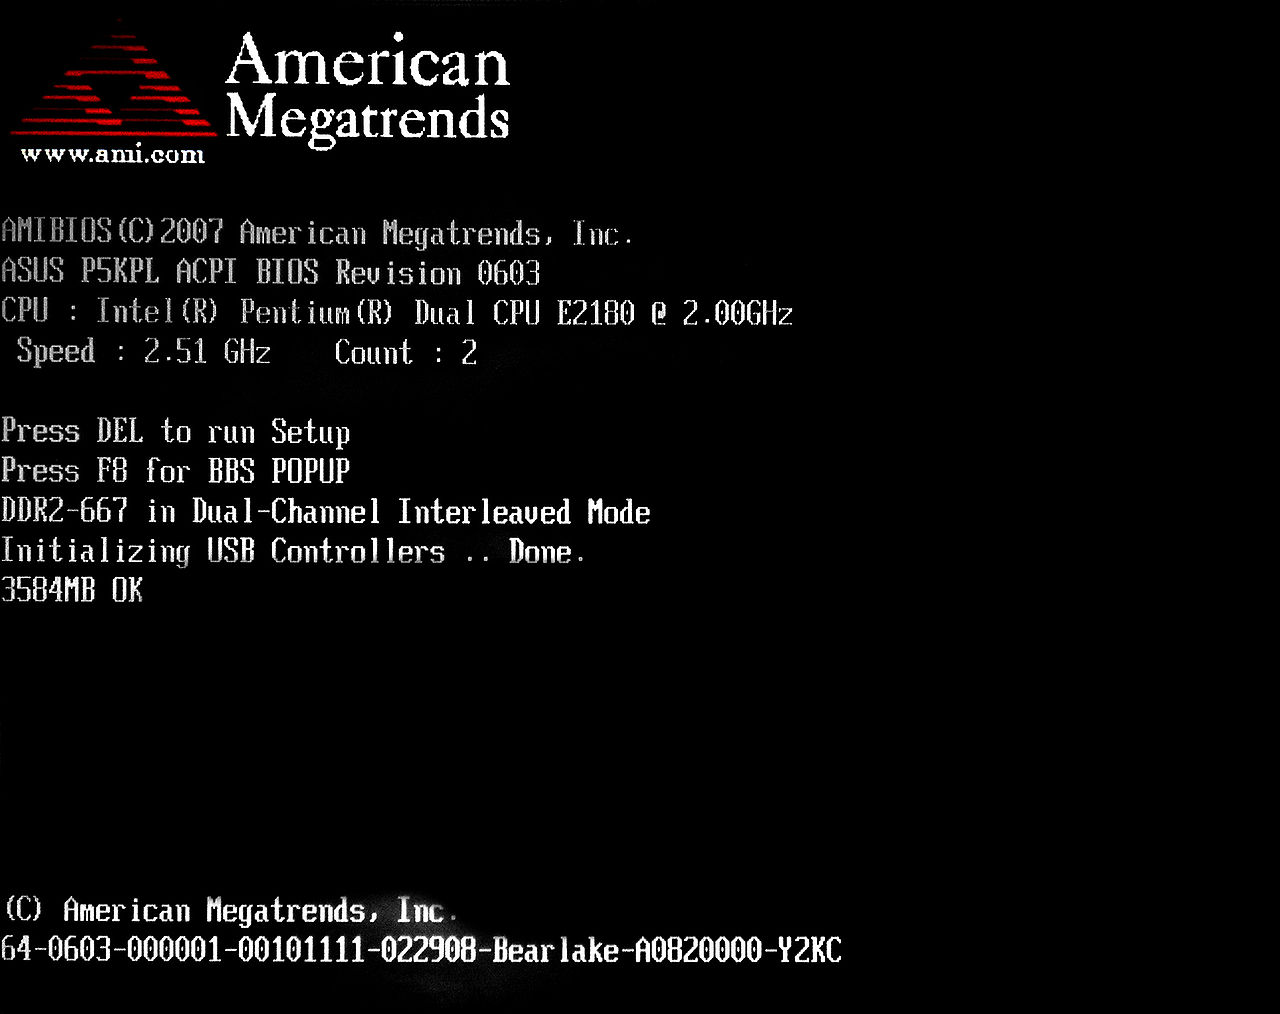
\includegraphics[width=.4\textwidth]{05/pics/POST}}
	\hspace{1em}
	\subfloat[Award Software BIOS]{\label{fig:software-installation:bios}
				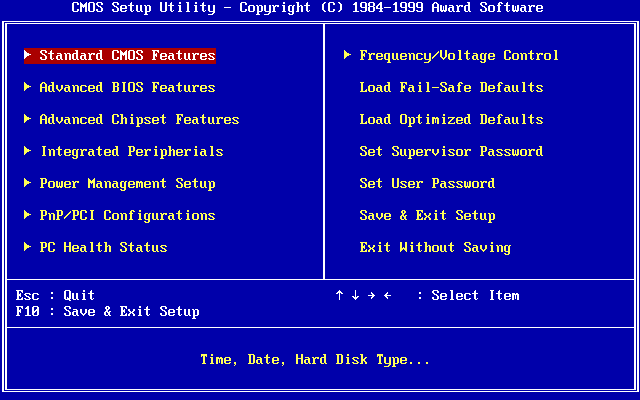
\includegraphics[width=.5\textwidth]{05/pics/BIOS}}
	\caption{A typical POST and BIOS screen}
\end{figure}

\begin{itemize}
	\item Power-On Self Test (\glslink{post}{POST}\index{POST}) -- a few very basic routines
		intended to insure the hardware is not obviously faulty;
		Figure \ref{fig:software-installation:post} shows a typical POST screen
	\item execution of the primary boot loader\index{boot loader!primary}
		-- a simple program stored in read-only memory; examples include
		the \gls{bios}\index{BIOS} (as shown in Figure
		\ref{fig:software-installation:bios}), \glslink{uefi}{UEFI}\index{UEFI},
		and OpenBoot\index{OpenBoot}/Open Firmware
	\item access of the \gls{mbr}\index{Master Boot Record} -- a special boot sector
		found on the primary boot device; the code found in this
		location allows the system to access the file system(s)
		and transfer control to a second-stage boot loader;
		see Chapter \ref{file systems:storage-models:dividing-and-combining-disks:partitions}
	\item execution of a secondary or second-stage boot loader --
		\index{boot loader!second-stage} a small program allowing
		the user to interactively choose an operating system or
		kernel to boot; examples include GRUB\index{GRUB} (Figure
		\ref{fig:software-installation:grub}) or
		{\tt boot(8)}\index{\tt boot(8)}
		(Figure  \ref{fig:software-installation:nbsdboot})
	\item loading of the hypervisor and starting
		of the privileged domain ({\em dom0}\index{Xen!dom0})
	\item initialization of the virtual hardware
		by the {\em domU} for the guest OS ({\em domU}\index{Xen!domU})
	\item loading of the guest OS kernel -- booting, initializing (virtual) hardware, loading
		modules
	\item \manpage{init(8)} -- one of the few processes created
		explicitly by the kernel, {\tt init(8)} spawns all other
		processes of the running OS and boostraps the final system
	\item starting of system services -- started by {\tt init(8)}, commonly via a
		number of shell scripts using e.g. the {\tt rc(8)}\index{\tt rc(8)} or
		{\tt /etc/init.d} frameworks
	\item the interactive system runs, presenting a login prompt; the web server
		accepts network connections and begins traffic
\end{itemize}

\newsavebox{\nbsdboot}
\begin{lrbox}{\nbsdboot}
\begin{minipage}{.7\textwidth}
\begin{lstlisting}[basicstyle=\scriptsize]
>> NetBSD/i386 BIOS Boot, Revision 5.2
>> (builds@b7, Sun Feb 7 00:30:50 UTC 2010)
>> Memory: 639/130048 k
Press return to boot now, any other key for boot menu
booting hd0a:netbsd - starting in 30
\end{lstlisting}
\end{minipage}
\end{lrbox}

\begin{figure}[t]
	\centering
	\subfloat[GNU GRUB]{\label{fig:software-installation:grub}
				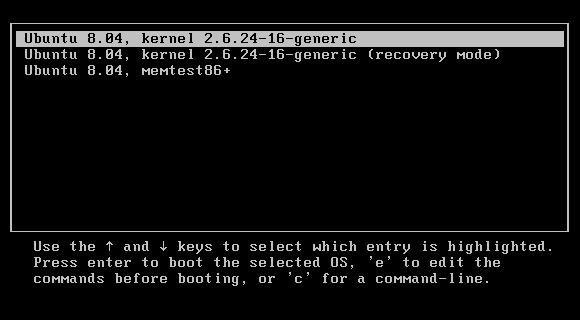
\includegraphics[width=.6\textwidth]{05/pics/grub}}
	\\
	\subfloat[NetBSD \manpage{boot(8)}]{\label{fig:software-installation:nbsdboot}
		\usebox{\nbsdboot}}
	\caption{Second stage boot loader examples}
\end{figure}

Most Unix systems display diagnostic messages from the
boot process on the system console\index{console} and
may retain a copy on the file system under e.g. {\tt
/var/run/dmesg.boot}.  The \manpage{dmesg(8)}
command can be used to display these messages.  On
Amazon's EC2 systems, you can use the {\tt aws ec2
get-console-output} command to retrieve the
information displayed on the (virtual) console.

Listing \ref{code:nbsdboot1} and \ref{code:nbsdboot2}
show the output on the serial console displayed during
the boot process of a NetBSD Amazon EC2
instance showing information from the hypervisor and
the virtualized guest OS respectively.

\begin{lstlisting}[float,basicstyle=\scriptsize,label=code:nbsdboot1,caption={Excerpt
of the boot messages of a NetBSD Xen
domU\index{Xen!domU} booting in
Amazon EC2}]
i-38d44816      Xen Minimal OS!
  start_info: 0xa01000(VA)
    nr_pages: 0x26700
  shared_inf: 0x7dcc4000(MA)
     pt_base: 0xa04000(VA)
nr_pt_frames: 0x9
    mfn_list: 0x967000(VA)
   mod_start: 0x0(VA)
     mod_len: 0
       flags: 0x0
    cmd_line: root=/dev/sda1 ro 4
  stack:      0x946780-0x966780
MM: Init
      _text: 0x0(VA)
     _etext: 0x61e65(VA)
   _erodata: 0x76000(VA)
     _edata: 0x7b6d4(VA)
stack start: 0x946780(VA)
       _end: 0x966d34(VA)
  start_pfn: a10
    max_pfn: 26700
Mapping memory range 0xc00000 - 0x26700000
setting 0x0-0x76000 readonly
skipped 0x1000
MM: Initialise page allocator for b3e000(b3e000)-0(26700000)
MM: done
Demand map pfns at 26701000-36701000.
Heap resides at 36702000-76702000.
Initialising timer interface
Initialising console ... done.
gnttab_table mapped at 0x26701000.
Initialising scheduler
Thread "Idle": pointer: 0x36702008, stack: 0xbf0000
Initialising xenbus
Thread "xenstore": pointer: 0x36702478, stack: 0x26600000
Dummy main: start_info=0x966880
Thread "main": pointer: 0x367028e8, stack: 0x26610000
"main" "root=/dev/sda1" "ro" "4" 
vbd 2049 is hd0
******************* BLKFRONT for device/vbd/2049 **********


backend at /local/domain/0/backend/vbd/1720/2049
Failed to read /local/domain/0/backend/vbd/1720/2049/feature-barrier.
Failed to read /local/domain/0/backend/vbd/1720/2049/feature-flush-cache.
2097152 sectors of 0 bytes
**************************
vbd 2050 is hd1
\end{lstlisting}

\begin{lstlisting}[float,basicstyle=\scriptsize,label=code:nbsdboot2,caption={Excerpt
of the boot messages of a NetBSD system}]
Copyright (c) 1996, 1997, 1998, 1999, 2000, 2001, 2002, 2003, 2004, 2005,
    2006, 2007, 2008, 2009, 2010, 2011, 2012
    The NetBSD Foundation, Inc.  All rights reserved.
Copyright (c) 1982, 1986, 1989, 1991, 1993
    The Regents of the University of California.  All rights reserved.

NetBSD 6.1.2 (XEN3PAE_DOMU)
total memory = 615 MB
avail memory = 597 MB
mainbus0 (root)
hypervisor0 at mainbus0: Xen version 3.4.3.amazon
vcpu0 at hypervisor0: Intel(R) Xeon(R) CPU E5-2650 0 @ 2.00GHz, id 0x206d7
xenbus0 at hypervisor0: Xen Virtual Bus Interface
xencons0 at hypervisor0: Xen Virtual Console Driver
npx0 at hypervisor0: using exception 16
xbd0 at xenbus0 id 2049: Xen Virtual Block Device Interface
xbd1 at xenbus0 id 2050: Xen Virtual Block Device Interface
xennet0 at xenbus0 id 0: Xen Virtual Network Interface
xennet0: MAC address 22:00:0a:47:89:0e
balloon0 at xenbus0 id 0: Xen Balloon driver
balloon0: current reservation: 629760 KiB
xennet0: using RX copy mode
balloon0: current reservation: 157440 pages => target: 157440 pages
boot device: xbd1
root on xbd1a dumps on xbd1b
root file system type: ffs
Sat Feb  1 21:46:17 UTC 2014
Starting root file system check:
/dev/rxbd1a: file system is clean; not checking
Starting file system checks:
/dev/rxbd0a: file system is clean; not checking
Setting tty flags.
Setting sysctl variables: ddb.onpanic: 1 -> 0
Starting network.
IPv6 mode: host
Adding interface aliases:.
Building databases: dev, utmp, utmpx, services.
Starting syslogd.
Mounting all filesystems...
Clearing temporary files.
Generating public/private rsa1 key pair.
Your identification has been saved in /etc/ssh/ssh_host_key.
Your public key has been saved in /etc/ssh/ssh_host_key.pub.
The key fingerprint is: ca:b3:e5:45:20:69:94:bf:ef:92:69:da:32:7b:1e:cc
Starting sshd.
Starting local daemons:.
Updating motd.
Starting powerd.
Starting inetd.
Starting cron.
Sat Feb  1 21:46:37 UTC 2014

NetBSD/i386 (ip-10-71-137-14.ec2.internal) (console)

login:
\end{lstlisting}

At each step of the boot process, we find a different
type of software active as the dominant component.  At
the final stage, when the system is up and running, we
can easily identify certain applications or services
that interact directly with the user.  This kind of
software does not require any special privileges and
does not rely on any particular hardware.  Even
though these applications may have a dependency on
specific features or capabilities in the OS, they are
effectively isolated from the kernel's privileged
execution mode.  They are entirely optional and
installed by the system administrator as needed;
common examples include a web browser or a database
management system.  In this book, we use the term
``add-on'' or ``third-party''
software\index{Software!Add-on}\index{Software!Third-Party}
to indicate that it was not included in or
distributed directly with the operating system.

Below these software packages exists a layer of
software applications and system utilities without
which the OS would simply not be complete.  All of the
common Unix utilities\index{Software!System Utilities}
such as \manpage{awk(1)} \manpage{sed(1)}, or even
\manpage{ls(1)} fall into this category, as do the
common system d\ae mons such as \manpage{sshd(8)} or
\manpage{syslogd(8)}, to name but a few.  The standard
Unix command interpreter, the shell, is part of this
layer, and most systems include a compiler chain and
other basic development tools as well.  Like add-on
software packages, this software also relies on a
number of basic OS capabilities, which form another
(sub-)category: the system libraries, kernel modules,
and device drivers used by applications to interact
with the OS kernel, the next layer in our software
stack.

We can define the kernel as the central component of
the operating system in charge of process-, device-
and memory management, facilitiating access to the
hardware via a small number of {\em system
calls}\index{system calls}.  Software running in the
kernel's address space has full access to all aspects
of the hardware and OS, while software running in
so-called ``user space'' relies on the kernel or the
system libraries to provide access to these resources
when needed.

Finally, we have a layer of software that falls
somewhat in between the kernel and the system
software: some of the physical resources maintained by
the kernel rely on hardware controllers providing
increasingly complex code running in persistent memory
on the devices themselves.  Since this software,
frequently consisting of low-level microcode, exists
somewhat in between the clearly defined categories of
{\em hardware} and {\em software}, it is commonly
referred to as {\em firmware}\index{firmware}.
Besides the previously mentioned RAID controllers or
Fibre Channel \gls{hba}, the most common example of
firmware here is probably the \gls{bios}.

Even though firmware can be viewed as residing
``below'' the kernel, closer to the hardware, many
systems provide tools to interact with or update the
firmware from within the OS.  Some of this software
requires the kernel to facilitate this access, for
example via a loadable module.  Likewise, the
previously mentioned bootloader is an independent
program executing outside the OS kernel, but from
within the OS we can manipulate its behaviour and
configure it to change the way the system is booted.

It is also worth mentioning that some code is executed
exactly once (POST, the bootloader), while other
low-level components (kernel modules or RAID firmware,
for example) are used periodically or continually
throughout a system's running time.  Once again, the
distinction between what constitutes optional add-on
software, an essential system component, or low-level
access to the hardware by the kernel is far from
obvious.

\subsection{Operating System vs. System Software vs. Third Party Software}
\label{software-installation:system-vs-third-party}
\index{Software!Distinction between different types of}

Our attempt to draw the software stack as described in
the previous section is illustrated in Figure
\ref{fig:software:types}.  As we review these layers,
it quickly becomes obvious that unfortunately the
distinctions are not as well-defined as we would like
them to be.

It has become increasingly difficult to clearly
identify any given piece of software as being an
``add-on package'', as OS providers include more and
more software in their distributions in order to make
their product suitable for the widest variety of uses.
Many Linux distributions, for example, include the
canonical examples cited above (web browsers, database
management systems, web servers, etc.), as they target
both the server and desktop markets, while the BSD
derived systems tend to favor a leaner setup,
explicitly targeting the server market.

But what exactly defines an operating system?  It is
clear that an OS cannot exist without a kernel, but on
the other hand a kernel all by itself does not provide
for a useful environment, either.  For this reason,
different providers bundle the kernel with {\em system
software} (device drivers, loadable kernel modules,
core libraries etc.) and {\em system utilities} (such
as a shell, the various command-line utilities, system
d\ae mons, development tools etc.).  The more closely
coupled these components are, the more coherent the
resulting OS is.  Many core system libraries rely on
the presence of certain features in the kernel, and
not keeping these components in sync or even replacing
one or the other tends to introduce a significant risk
of instability.

For this reason, many OS providers only support their
own specific releases of the many system components in
their specific software bundle.  If you replace parts
of the system (either the kernel, core libraries, or
various important system components), you are breaking
up the bundle of software that initially made up the
given release of the OS in question.  You are in
effect creating a different version, a different
``distribution'' of the OS.\footnote{ Nowadays, the
term is more commonly used when referring to a
specific Linux flavor, but recall from Chapter
\ref{unix:history:os} that the ``D'' in ``BSD'' stands
for ``distribution'': the idea of bundling different
software packages and making them available as a
well-defined release has been around for quite some
time.}

Many Unix versions come in only exactly one flavor,
one bundle of kernel plus libraries plus system
utilities -- the open source BSD versions and
virtually all of the ``old'' commercial Unix versions
fall into this category.  Releases differ across time
in features added or removed, but a given version of
the OS will behave the same way anywhere you may
encounter it.

Contrast this with the world of Linux, where the
definition of a coherent operating system has been
replaced with variety in software bundling: a common
kernel (possibly with custom modifications) combined
with the core libraries from the \gls{gnu} project and
a suprising variety of different add-on software.
Some of these ``distributions'' replace core system
utilities, some remove components but add others etc.,
until they behave sufficiently different from one
another that they may well be regarded as unique Unix
flavors.  \\

\begin{figure}[t]
	\centering
	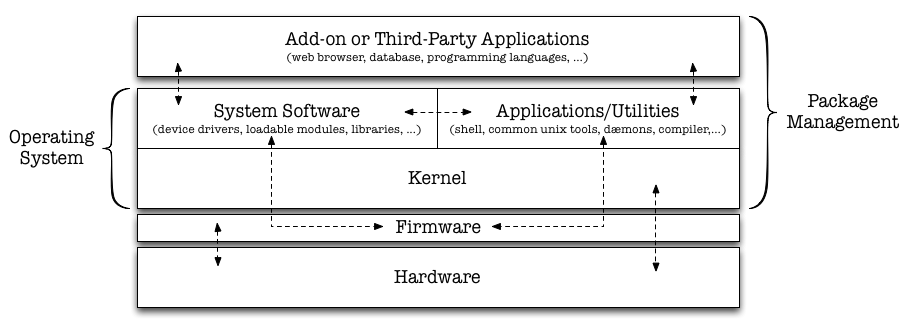
\includegraphics[width=.85\textwidth]{05/pics/types-of-software}
		\caption[Types of Software]{We define a software layer
			stack consisting of ``Add-on Applications'',
			``System Software'' and
			``Applications/Utilities'', the kernel, and
			firmware, some of which may be controlled via a
			package management system.  Interactions between
			these types are illustrated as arrows, but it is
			important to note that none of these distinctions
			are precise.
			\label{fig:software:types}}
\end{figure}


As different OS providers disagree on what components
should be part of their final product, it becomes very
difficult to declare a software package to belong into
any one of the categories we've defined.  However,
most system administrators ultimately develop an
instinctive idea of what should or should not be
considered {\em essential}, what can and cannot be
removed from the system without unexpected side
effects, and which components may only be upgraded in
sync with kernel- or system library upgrades.

This understanding comes with years of experience, and
it helps to think about software in terms of their
place in the software stack we have defined.  As so
often, we end up creating flexible definitions that
allow us to translate core concepts across variable
implementations.  We will see throughout this chapter
how this approach will help us understand the
installation- and upgrade process, the placement of
software within the file system hierarchy, how system
configuration files and software runtime changes are
handled and hopefully gain a better understanding of
how to tune and maintain our systems.

\section{File System Layout}
\label{software-installation:file-system-layout}

In Section \ref{file systems:layout}, we briefly
summarized the hierarchical tree-like structure of the
Unix file system layout and noted that the purpose or
common use of the different subdirectories as
described on many Unix versions in the {\tt hier(7)}
manual page.  Unfortunately, this layout is not
standardized and different versions of Unix have, for
historical reasons as well as purely by coincidence or
developers' preferences, diverged.  But almost all
Unix versions do still share a number of common
directories, especially as far as the base OS is
concerned.

In the early days of Unix, disk space was still
expensive, and it was not uncommon to split the files
of the operating system across multiple devices.  As
the system boots up, it obviously requires a number of
files to be present and services to run before it can
mount any other partitions or disks.  For this reason,
Unix systems used to have a small root partition
(mounted at {\tt /}, pronounced ``slash''), sufficient
to boot the OS, with additional software stored on a
separate disk, commonly mounted under {\tt /usr}.
{\tt /} contained all the system binaries (found in
{\tt /bin}) and libraries (found in {\tt /lib}) to
perform basic system maintenance, while so-called
``user'' binaries and libraries were found in {\tt
/usr/bin} and {\tt /usr/lib} respectively; the use of
the different {\tt bin} and {\tt lib} directories
themselves already hints at a clear definition of
purpose.

Since costs for disk space have come down so far as to
no longer be a limiting factor, it is nowadays rare to
find a Unix system that actually has {\tt /usr} on a
separate device from the root partition.
Nevertheless, this historical distinction remains
useful: it illustrates careful forethought with
regards to the placement of and interactions amongst
software components, which is worth reviewing in
detail.  Listing \ref{code:hier} shows an excerpt of
the \manpage{hier(7)} manual page on a NetBSD system.  The
definitions there overlap with those given in the
``Filesystem Hierarchy Standard''\index{Filesystem
Hierarchy Standard}\cite{fhs}, a formalization of this
same old hierarchy overseen by the Linux
Foundation\index{Linux Foundation}.

\begin{lstlisting}[float,basicstyle=\scriptsize,label=code:hier,caption={Excerpt of the {\tt hier(7)} manual page.}]
NAME
    hier -- layout of filesystems

DESCRIPTION
    An outline of the filesystem hierarchy.

    /          root directory of the system

    /bin/      utilities used in both single and multi-user environ-
               ments

    /etc/      system configuration files and scripts

    /lib/      dynamic linked libraries used by dynamic linked programs
               (such as those in /bin/ and /sbin/) that cannot rely
               upon /usr/lib/ being available.

    /libexec/  system utilities (such as the dynamic linker) required
               by programs and libraries that cannot rely upon
               /usr/libexec/ being available.

    /sbin/     system programs and administration utilities used in
               both single-user and multi-user environments


    /tmp/      temporary files, usually a mfs(8) memory-based file
               system (the contents of /tmp are usually not preserved
               across a system reboot)

    /usr/      contains the majority of the system utilities and files

               bin/      common utilities, programming tools, and
                         applications

               lib/      archive, profiled, position independent
                         archive, and shared libraries

               libexec/  system daemons & system utilities (executed
                         by other programs)

               sbin/     system daemons and system utilities
                         (normally executed by the super-user)

               share/    architecture-independent text files

    /var/      multi-purpose log, temporary, transient, and spool files

               log/      miscellaneous system log files

               run/      system information files, rebuilt after each
                         reboot

               tmp/      temporary files that are not discarded
                         between system reboots

SEE ALSO
     apropos(1), ls(1), whatis(1), whereis(1), which(1), paths(3)

HISTORY
     A hier manual page appeared in Version 7 AT&T UNIX.
\end{lstlisting}

Due to the previously mentioned traditional separation
of {\tt /} and {\tt /usr}, it is not surprising to see
a similar subtree reflecting the root file system
under {\tt /usr}.  That is, we find subdirectories
named {\tt bin}, {\tt lib}, {\tt libexec}, {\tt sbin}
and {\tt share}, with each having a similar purpose as
under the root.  On many systems, we also find the
{\tt /usr/local} directory as a specific location for
files that are not part of the base OS.  This
directory has become the default location for any
``add-on'' software, and it is thus not very
surprising that it also mirrors the general root
hierarchy to some extent.

Note that {\tt /usr} contains a subdirectory named
{\tt share} for so-called ``architecture independent
data-files''.  As the name suggests, the files in this
location are intended to be able to be shared across
multiple system.  Another directory with a
particularly descriptive name is {\tt /var}, for
``variable'' or transient data, known to change at
runtime.

These two directories already hint at two major
properties of files found on any Unix system, each
with distinct implications on where or how they might
best be organized\cite{fhs}, and each deriving from
standards and best practices of the early days of
Unix: \\

{\bf Shareable} versus {\bf unshareable} content:
Data files that remain the same across multiple hosts,
and, as the manual page suggests, possibly even across
different hardware architectures are considered {\em
shareable}.  Flat text files or simple system
databases that are not used for runtime configuration
such as manual pages, timezone or terminal
information, are good examples.\footnote{It should be
noted that across hosts of a uniform hardware
architecture most binaries are also common candidates
for shareable directories, and it was, in fact, not
uncommon for multiple hosts to share {\tt /usr}, for
example.  Nowadays, such a setup is a rare exception.}
This data frequently remains unchanged throughout
day-to-day operations -- that is, it only changes if
it is intentionally and specifically updated.  Note
that these files may at times overlap with some
``local'' data (i.e. files not included in the base
OS).

Data files that need to be individual to each host are
considered {\em unshareable}.  Sometimes this is due
to the fact that the data simply changes at runtime
(such as a sytem's log files), other times it is
because these files define a unique feature of a given
host (most files under the {\tt /etc} directory fall
into this category).  Note that once again these files
may at times overlap with certain ``local'' data.  \\

{\bf Static} versus {\bf variable} data:  Files that
are not expected to change during the runtime of the
system are considered {\em static}.  This includes the
kernel, all system libraries and binaries and many
data files.  Note that these files may, of course, be
changed when the system is upgraded, for example, but
are not modified under normal circumstances.

Files that are updated by the OS, by any running
applications or by end-users at runtime, are termed
{\em variable}.  That is, we anticipate that these
files will be created, modified, updated, or removed.
Some may see frequent or even continous updates (such
as the various log files), while others only see
comparatively rare modifications (such as when a
system d\ae mon is restarted).  \\

Combining these four classes of data yields a matrix
of files with common locations in the file system
hierarchy as illustrated in Table
\ref{table:software-installation:shareable-variable}.
Note that not all static data is necessarily
shareable, just as not all variable data is
necessarily unshareable.

\begin{table}[b]
\centering
	\begin{tabular}{ l l l }
	& shareable content & unshareable content \\
	\hline
	static data & {\tt /usr} & {\tt /boot} \\
	& {\tt /opt} & {\tt /etc} \\
	\hline
	variable data & {\tt /var/mail} & {\tt /var/run} \\
	& {\tt /var/spool/news} & {\tt /var/lock} \\
	\hline
	\end{tabular}
	\caption[Shareable/unshareable vs. static/variable files]{Typical
		examples of shareable/unshareable vs. static/variable files.}
	\label{table:software-installation:shareable-variable}
\end{table}

Even though nowadays it is less and less common for
multiple Unix system to share specific directories or
mount points (perhaps with the exception of users'
home directories, which are still frequently accessed
over a network file system), the distinction of
variable versus static data is of particular
importance.  Carefully separating these kinds of data
will allow you to build systems with separate mount
options for these types, which can improve performance
and security significantly.  As examples, consider a
read-only partition for system binaries to prevent
accidental or malicious writes to the base OS, or
mounting a directory containing system logs using the
{\tt noatime} or {\tt noexec} mount
options.\footnote{Reference your \manpage{mount(8)} manual
page for details.  Many other options are available.}

Understanding these criteria also helps make sense of
why software providers choose a certain location for
their files, or how different package managers may
apply the file system hierarchy standard.  Beware,
however, that not all software providers necessarily
understand or follow this matrix or even the general
Unix conventions!

\section{OS Installation}
\label{software-installation:os-installation}

System administrators often maintain large numbers of
hosts, and so it comes as no surprise that new
machines -- both physical and virtual -- have to be
brought up and integrated into the infrastructure on a
regular basis.  The more systems are maintained and
created, the more this process needs to be automated,
but at the end of the day, each one follows the same
set of common steps.  In an ideal world, these steps
could be summarized as requiring the installation of a
base operating system with subsequent adjustments for
the specific task at hand.

As we will see in this section, each step depends on a
large number of variables and site-specific
customizations, and so most large-scale organizations
have written their own automation framework around a
few common tools to accomplish the goal of quick and
scalable system and service deployment.  In fact, the
topic of automated deployment tools is too large to
adaequately cover here (though we will revisit it in
later chapters) and we shall instead focus on the
essential concepts needed to understand the
requirements for such systems.

Installing a new system is a process unique to each
OS; installation methods range from unattended
deployment systems using information determined at
runtime to create the correct configuration to
interactive graphical installers (such as seen in
Figure \ref{fig:os-installation:opensolaris}) allowing
users to select amongst common options to create a
general purpose Unix server.  Understanding the
individual steps included is valuable, and we
recommend strongly for students to perform this task
as a learning exercise (see Problems
\ref{prob:software-installation:os-installation} and
\ref{prob:software-installation:os-installation:manual}):
sooner or later, any system administrator will find
him or herself trying to debug a broken installation,
and understanding all the steps performed and what
things might have gone wrong in the process are
invaluable.

\begin{figure}[t]
	\centering
	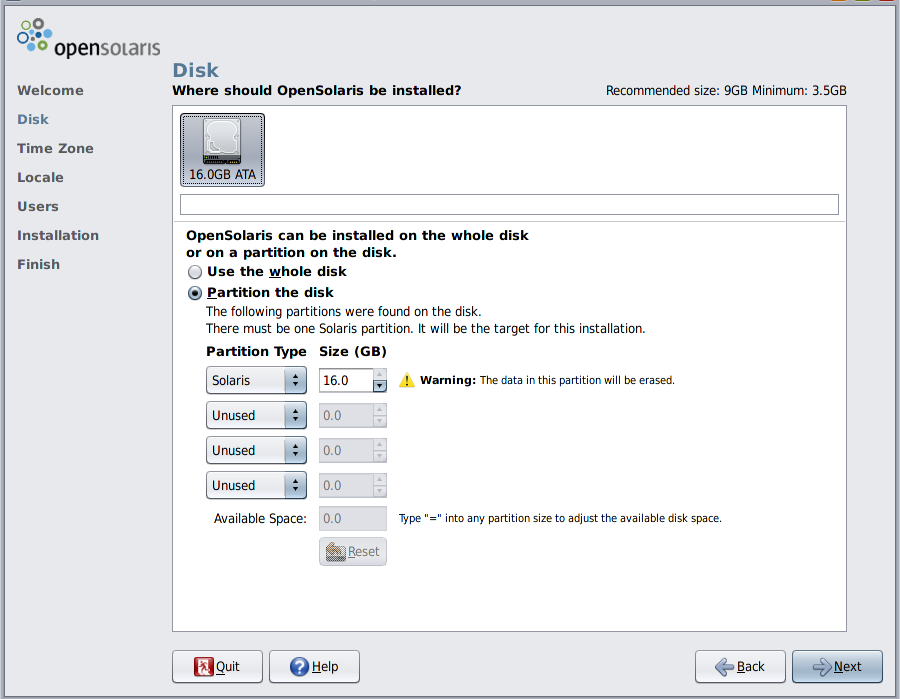
\includegraphics[width=.85\textwidth]{05/pics/opensolaris-install}
		\caption[OpenSolaris Installation]{A graphical installer
			showing an interactive disk partitioning tool.
			\label{fig:os-installation:opensolaris}}
\end{figure}

\subsection{Identifying server requirements}
\label{software-installation:os-installation:requirements}

Before a system is installed, a number of important
choices have to be made: What file system will be
used?  What are the requirements of the final system
with respect to file I/O?  How many partitions will be
created?  What OS will be installed?  What add-on
software?  What is the final purpose of the machine?

Many of these questions are interdependent and
answering one may restrict possible answers to other
questions.  For example, if the purpose of the server
is to run a specific piece of software that is only
available for a given OS, then this might also
influence a very specific partitioning schema or other
file system considerations.  In fact, the final
purpose of the machine and the software it needs to
run will likely dictate your hardware choices --
processor architecture, amount of memory and disk
space, number or types of network interfaces -- which
in turn restrict your OS choices.

For example, if you plan on building a highly
performant database server able to handle a large
number of transactions per second, you can quickly
identify the number of CPUs and CPU speed needed, the
size of RAM to provide a large in-memory buffer cache,
as well as hard drive disk speed and network
throughput requirements, but not all operating systems
are able to handle with equal efficiency the same
amount of CPUs, RAM, or perhaps link
aggregation\index{link aggregation}, for example.  As
a result, your database server may {\em have to} run
e.g. Solaris, even though the rest of your hosts are
all running Linux (or vice versa).

On the other hand, it is possible that the cost of
running a different OS just for one purpose is not
worth the benefit of running the theoretically ideal
software.  Instead, you might prefer to change your
infrastructure architecture and perhaps scale the
database horizontally across a number of smaller
commodity hardware systems to meet the requirements.
Whichever approach you choose, these design decisions
need to obviously be made prior to the OS installation
itself -- changing your OS later on often results in
much higher costs, as services have to be migrated,
ported, and verified while the server is already in
production use, a process that has been likened to
changing one's tires on a car travelling on a busy
highway at 100 miles per hour.

\subsection{OS Installation Overview}
\label{software-installation:os-installation:overview}

On a high level, the OS installation process itself consists of a few
distinct phases:

\begin{itemize}
	\item {\bf Hardware identification, provisioning and registration.}
		Before a new system can be installed, suitable hardware
		needs to be identified, physically installed, and
		registered with the inventory system.  Depending on the
		size of your organization, this may be a manual step
		performed immediately before the OS installation is
		started, or it might be done continously in a data center
		where hardware is racked, asset tags scanned and
		information automatically entered into a pool of
		``ready to install'' systems.

	\item {\bf Base OS installation.}
		The installation of the software itself.  Even though
		any reasonable deployment system combines these steps,
		we distinguish between the basic OS and additional
		software added (or unused components removed), to more
		clearly illustrate at which point in the process
		customization to our needs tends to happen.

	\item {\bf Installation of add-on applications.}
		In this step, we transform the generic OS into a server
		with a specific purpose.  The installation of the right
		add-on applications may entail fetching software updates
		over the network from a remote system or even building
		binaries from sources on the fly.

	\item {\bf Initial minimum system configuration.}
		After all software has been installed, a number of very
		basic configuration steps have to be performed.  This
		phase may include setting a hostname, applying a specific
		network configuration, adding user accounts or enabling
		certain system d\ae mons.  Note that in most cases a {\em
		configuration management system}\index{Configuration Management} is installed, which
		will perform this (and then ongoing) customization.

	\item {\bf System registration.}
		When all software is installed and configured and the system
		is ready to run and fulfill its purpose, we need to integrate
		it into our larger infrastructure.  Our inventory of which
		systems perform which function needs to be updated, our
		monitoring system needs to be made aware of this host, other
		components with which this server interacts may need to be
		updated etc.  It is important to consider this
		``paperwork'' to be part of {\em installation}, lest it be
		deprioritized or forgotten.

	\item {\bf System restart.}
		Finally, the system needs to be rebooted at least once
		before it is put into service.  This ensures that it can
		boot off the right media, all d\ae mons start up, the
		network is functional, the system can be monitored and in
		general everything behaves exactly as it should.  It is
		important to always include this step: during the
		installation process the system is in a very different
		state than under normal circumstances, and it is possible
		to forget to enable or disable a service.  Placing the
		system into production use without a fresh reboot might
		lead to unexpected results when the system is rebooted at
		a later point.
\end{itemize}

Obviously, each of these steps consists of many
smaller substeps; how exactly each of these main
objectives is accomplished depends heavily on the size
of the organization, the resources available, and the
level of automation required.  In addition, there is a
thin line between {\em system deployment}\index{system
deployment} and {\em system configuration}.  As
mentioned, the OS installation always includes at the
very least a few minimal configuration steps, but some
of the steps noted above may be considered part of a
configuration management system's first run.  That is,
much like the distinction between add-on software and
core system components, there exists a discrepancy
between what aspects of a server's configuration are
to be defined at installation time and which ones are
dynamically determined at runtime.  We will cover this
in more detail in Chapter
\ref{chap:configuration-management}; for the time
being, let us merely state that one way or another the
system, once completely installed and set up, is
configured for its final purpose.

\begin{experience}
{\bf Magic Deployment} \\

Around early 2007, during my time at Yahoo! Inc., I
worked together with a number of people on a
deployment system suitable to quickly build new Unix
systems and bring them up, ready to serve production
traffic.  As so many other shops, we, too, chose to
develop our own solution instead of using an existing
commercial or open-source system for this purpose.
Our setup was ``special'', unique, different from
whatever the existing solutions provided -- just like
everybody else's. (For what it's worth, this also
well predates scalable deployment engines and other
\gls{iaas}\index{Infrastructure!As a Service}
solutions such as e.g. OpenStack\index{OpenStack}.) \\
[10pt]

As a friend of mine once remarked,
you're not truly a system administrator until you have
written your own deployment system. Or configuration
management system.  Or inventory database.  Or
parallel secure shell to perform tasks across all of
your host.  Or... \\ [10pt]

Anyway, the system we wrote was elegant, and it taught
us a lot about the details of the OS installation
process.  Our goal was to allow hardware to be
delivered to the datacenter, be physically racked and
their asset tags scanned, and then not require any
more physical contact to be deployed, while at the
same time allow existing systems to be rebuilt or
decommissioned as needed. \\ [10pt]

Our final solution used IPMI\index{IPMI} to power on
the host, DHCP\index{DHCP} to assign a system {\em
profile} to the hardware (derived from a central
database, where the system was identified by the asset
tag), and a {\tt pxeboot}\index{pxeboot} process to
run the system through a number of stages.  In the
initial stage, the system would power up, identify and
apply any pending firmware upgrades, and then check if
it was ready to be deployed.  If not, it would go into
a special ``inventory'' state and power down. \\
[10pt]

When a number of hosts (frequently in the order of
tens or hundreds) had to be deployed, the system would
select suitable hardware from the pool of
``inventory'' systems, power them on, send them
through the initial stage again -- since it was
possible that a lot of time had passed since they were
first provisioned, additional firmware updates might
have been necessary -- and then enter the OS-specific
installation phase. \\ [10pt]

In this phase, the server was configured for its final
purpose: the correct OS and network configuration was
installed, software packages were deployed according
to the systems' profiles, user accounts added and
finally the system registered in the central database
as being ready for production traffic. \\ [10pt]

We programmed this system from afar, but the first
time we went to a datacenter to see it in action, we
were pleasantly surprised how well it worked: without
any physical interaction, we could see racks of
servers suddenly power up, install, reboot and start
taking traffic based on a simple hardware provisioning
request. \\ [10pt]

Arthur C. Clarke\index[names]{Clarke, Arthur C.} once remarked
that ``any sufficiently advanced technology is
indistinguishable from magic'', and so we proudly
named the project ``Magic Deployment''.  Three years
later, the system was obsoleted by a new, more
flexible system, re-written from scratch, ready to
adapt to the evolving requirements of this large
company...
\end{experience}

\subsection{OS Installation Details}
\label{software-installation:os-installation:details}

The list of phases outlined in the previous section
can be further refined.  It is clear that a number of
these steps are likely (and necessarily) dependent on
and intricately intertwined with a number of your
organization's infrastructure components, such as an
inventory system or a database keeping track of
configuration types or service roles, for example.

This integration into the larger infrastructure
ecosystem of a company tends to be complicated, which
is why most of these organizations end up writing
their own custom software for this purpose.  However,
eventually all of these systems, be they custom,
proprietary, public, open source, developed by the OS
provider or by a third party -- all of them have to
perform the same basic steps to actually get the OS
onto the disks.  Most installers hide the details of
these steps from the ordinary end-user, but, hey,
we're system administrators -- let's take a look under
the hood!  \\

\begin{enumerate}

	\item {\bf Boot the system.}\footnote{Note:
		with an eye towards security, we
		should mention in this context the
		concepts of {\em trustworthy
		computing}\index{trustworthy computing} and
		e.g. {\em hardware attestation}\index{hardware attestation},
		which may provide assurance that the
		system has not been tampered with
		prior to our booting it.  We will
		revisit this important topic in some
		detail in Chapter
		\ref{chap:security}.}
		This entails a decision of which
		media to boot from.  Manual installations tend to be
		performed by booting from a CD/DVD, while automated,
		unattended installs have for years relied on booting
		the system from the network using the {\em \gls{pxe}},
		\index{PXE}\index{pxeboot}
		which utilizes a combination of protocols such as {\em
		DHCP}, {\em TFTP}, {\em NFS} and/or memory-based
		filesystems to load a small version of the OS -- such as,
		for example, the Linux {\em initial ramdisk} ({\tt initrd(4)}) --
		which then performs all the steps to actually install the final
		system.

	\item {\bf Identify disk(s).}  Once booted, the install
		process needs to identify all available disks.
		This requires the ``miniroot'' to include or be able to load
		any drivers required to access the storage devices in
		question.

	\item {\bf Create partition table(s).}  Before the system can be
		installed, the disks identified in the previous step need
		to be partitioned.  This includes both the creation of a
		suitable \gls{bios} partition table (via e.g. \manpage{fdisk(8)}
		and/or the OS-specific disk label such
		as \manpage{disklabel(8)}).  At this step, we also need to
		decide on which of the available disks will become the
		target root device, i.e. which will contain the root
		file system, and where the other disks and partitions will
		be mounted later on.

	\item {\bf Create file system(s).}  Each partition defined in the
		previous step needs to be formatted for its respective
		file system.  It is important to pass the correct flags to
		\manpage{mkfs(8)}/\manpage{newfs(8)} since, as we
		discussed in Section \ref{sec:unix-file-system}, most file
		system features cannot (easily) be tuned at run time.

	\item {\bf Make the system bootable.}  At some point after the disks
		have been partitioned and before the host is rebooted for
		the first time, it needs to be made bootable.\footnote{The order
		of this step is not important, but leaving it out
		will yield a server unable to start up without
		manual intervention.}  The details depend again on the OS
		in question, but generally involve the installation of the
		disk bootstrap software in the \glslink{mbr}{MBR}\index{Master
		Boot Record} and the configuration of the first and second
		stage boot loader, for example via \manpage{installboot(8)} or
		\manpage{grub(1)}.

	\item {\bf Install the OS.}  Finally we have reached the point
		where the actual OS is installed.  This generally requires
		the retrieval of the system's base packages or archive
		files from a CD or DVD, via \gls{nfs} from another server or
		(perhaps via FTP) from a remote host (an approach which
		brings with it a number of security implications --
		how do you verify source authenticity and integrity? --
		and in which case initial network configuration of the
		miniroot system is a pre-requisite).

		After the data files have been retrieved, they are
		extracted or the necessary packages installed into the
		target root device.  Many interactive installers allow the
		user to select different sets of software to install
		and/or will automatically identify additional packages as
		required.

	\item {\bf Install add-on software.} After the base OS has been
		installed, any optional software may be added, based on
		either the system's configuration or interactive user
		input.  Depending on the installer, this step may be
		combined with the previous step.  We explicitly note this
		as a separate step, since ``add-on'' software here may not
		only include optional packages from our OS vendor, but
		also your own software, such as your configuration
		management system, third-party applications licensed to
		your organization, or your software product or serving
		stack.

	\item {\bf Basic system configuration.}  As we mentioned before,
		any server requires ongoing maintenance that, in large
		part, is performed by automated systems performing
		configuration management.  But regardless of whether or
		not such a (complex) system is integrated into the OS
		installation process, there are a few things that need to
		be defined at install time.  This usually includes
		a host's network configuration and hostname, timezone, NTP
		and syslog servers, root password, and services started at
		boot time, to name just a few examples.

	\item {\bf Reboot.}  Finally, after the system has been installed
		and basic configuration performed, it needs to be
		rebooted.  At this time, the host boots the way it would
		under normal circumstances and enters a ``first boot''.
		This stage in a host's deployment process tends to be
		significantly different from a normal boot:  a number of
		services are run for the first time, and further initial
		system configuration and system registration (as noted
		above) is likely to take place.

		Since this initial boot sequence may install software
		upgrades and change the runtime configuration, it is
		advisable to reboot the host {\em another} time
		after this ``first boot''.  This ensures that the system
		does in fact come up in precisely the same state as it
		would in the future.

\end{enumerate}

Listing \ref{code:netbsd-install} shows the most basic
steps to perform a minimal OS installation.  It is
interesting to analyze each of them (and constrast the
sequence for different operating systems), as doing so
often illustrates a number of assumptions made about
the use of the software.  The ease with which an OS
installation can be automated (at scale!) shows how
much the OS provider has prepared their system for a
wide variety of use cases.  System defaults, such as
what services are enabled and started by default,
speak volumes about general design philosophies.
Similarly, the selection of software bundled with the
OS reflects on the target audience for a given OS.

Deploying a new host requires more than just
installing an operating system, however.  The system
needs to be incorporated into our larger
infrastructure, which may entail updates to a number
of inventories or databases that keep track of an
organizations assets or the various hosts' purposes.
This integration is necessarily very different from
site to site and unfortunately frequently not suitably
abstracted into a general \gls{api} that an installer
might integrate with.  As a result, most system
administrators do end up writing their own deployment
system and/or helper tools, calling into the various
operating systems' specific installers, and adding
their own customizations.

One of the many customizations included in any
software deployment system includes the extent to
which add-on software is controlled.  Getting the
right software onto the machine is part of the
installation process, but there is more to managing
applications and configuration files than copying
files from one place to another.  In the next section,
we will take a closer look at this topic.

\begin{lstlisting}[float,basicstyle=\scriptsize,label=code:netbsd-install,caption={[Commands
used during the installation of NetBSD]Manual
installation of NetBSD using the \manpage{fdisk(8)},
\manpage{disklabel(8)}, \manpage{newfs(8)}, and
\manpage{installboot(8)} commands.}]
# fdisk -f -u -0 -s 169/63/4194241 /dev/rwd0d
# fdisk -f -c /usr/mdec/mbr /dev/rwd0d
# fdisk -f -a -0 /dev/rwd0d
# disklabel -e -I wd0
[...]
4 partitions:
#      size   offset fstype [fsize bsize cpg/sgs]
a:  4194241       63 4.2BSD    0     0      0 # (Cyl.      0*- 4161*)
c:  4194241       63 4.2BSD    0     0      0 # (Cyl.      0*- 4161*)
d:  4194304        0 unused    0     0      0 # (Cyl.      0 - 4161*)
# /sbin/newfs -O 2 /dev/rwd0a
/dev/rwd0a: 2048.0MB (4194240 sectors) block size 16384,
        fragment size 2048 using 12 cylinder groups of
        170.67MB, 10923 blks, 21504 inodes.
super-block backups (for fsck_ffs -b #) at:
32, 349568, 699104, 1048640, 1398176, 1747712, 2097248, 2446784,
....................................................................
# mount -o async /dev/wd0a /mnt
# for pkg in base comp etc games man misc modules text kern-GENERIC; do
        tar zxpf /i386/binary/sets/${pkg}.tgz -C /mnt
done
# cp /mnt/usr/mdec/boot /mnt/boot
# /usr/sbin/installboot -v -o timeout=5 /dev/rwd0a \
        /mnt/usr/mdec/bootxx_ffsv2
File system:       /dev/rwd0a
Primary bootstrap: /usr/mdec/bootxx_ffsv2
Boot options:      timeout 5, flags 0, speed 9600, ioaddr 0, console pc
# cd /mnt/dev && ./MAKEDEV all
# shutdown -r now
\end{lstlisting}


\section{Package Management Systems}
\label{software-installation:package-management}

Even though software installation methods across
different Unix versions can generally be achieved
using the same set of manual commands, most
third-party software is added using the operating
system's native package management tools to ensure a
tight integration with the OS as well as a consistent
and predictable file system hierarchy.

As we discussed earlier, almost all Unix systems have
a distinction between what they consider to be part of
the ``base OS'' and what is considered an ``add-on''
application.  For some versions, such as the BSD
derived systems, this distinction is clear and extends
to the way that the software is installed and
maintained:  the core operating system is provided in
software archives or built from source, while all
other software is installed through the use of a set
of specific, native tools managing a system-wide
package inventory.

Other Unix versions take a different approach: in
order to better express software dependencies on the
OS and its capabilities, as well as to make it easier
for system adminsitrators to manage {\em all}
software, including OS or core-component upgrades
using the same set of tools, they break all software
into individual packages.  This provides the benefit
of a more consistent user experience in controlling
software across all layers of the stack, but it is
easy to lose the distinction of which parts are
essential components of the operating system, and
which are optional.  As many vendors strive to provide
an OS suitable for many different purposes,
including as a general Unix workstation, a desktop
system, or a web server, more and more software is
included in a given OS release -- a lot of it
unnecessarily so.

\subsection{``Manual'' Software Installation}
\label{software-installation:package-management:manual}

Regardless of which package management system is
provided by the OS vendor, across all Unix versions
system administrators may at times choose to install
software ``by hand'', that is, by manually downloading
and possibly building the software before copying it
into the desired location.  With a plethora of
available open source software, it is the rule more
than the norm that an application you wish to install
is available only in source form, not as a binary
package.  The sequence of commands to install most
such software ({\tt ./configure; make; make install})
has become a ubiquitous part of a system
administrator's life, but unfortunately this approach
does not scale well:  a package management system not
only {\em installs} software, but, as the name
suggests, {\em manages} it.  That is, it provides tools
that can identify which files belong to which package,
that allow you to delete a package (and only do so if
the files provided by this package are not required by
other software), and to pull in additional software to
meet prerequisites.\footnote{Commercial software tends
to be provided in binary packages, where one does not
have the liberty to configure either its prerequisites
or final installation destination.  We still have to
identify and ensure the availability of all software
that this product relies on.}

Nevertheless, at times there are good reasons to choose a manual
installation method, if only for evaluation purposes of the software or
perhaps as a first step prior to deployment on a larger scale.  These
include:

\begin{itemize}
	\item {\bf Availability.}  There are tens of thousands of
		applications and libraries available, but not all software
		providers package their software.  In other
		words, you may simply have no choice but to (initially)
		build the software from source by hand.

		Nowadays a lot of software developers target almost
		exclusively specific Linux versions for their releases, so
		that even if a package may exist for this platform, you
		still have to build your own if you are running any other
		system.

	\item {\bf Customization and Optimization.}  By using pre-compiled
		binary packages, you give up a certain amount of control
		over the installed software.  When building 
		from source, you have the option to specify configuration
		options (such as including support for certain features
		normally disabled) or to create executables that are
		specifically optimized for your target platform.

	\item {\bf Adding Support for your OS.}  Sometimes software
		provided to you will not work correctly, not work
		at all, or not even build on your specific OS\footnote{A
		famous quote, often referred to as {\em
		Sturgeon's revelation}\index{Sturgeon's Law}, says: ``90\%
		of everything is crud.'' It refers to the
		fact that within any domain, only a small percentage of
		the work exhibits excellence.  This most certainly seems to
		hold for software, and if you are not running the most popular and
		latest Linux version, you often find yourself having to patch and
		fix the software you are installing.}.  With access to
		the source code, you can -- often with minimal effort -- port
		the software to your platform.

	\item {\bf Adding/removing features.}  Binary packages are built
		to target the largest user base possible.  As a result,
		they tend to include built-in support for all possible
		features, including those that you may not have any use
		for or that may actually be undesirable in your
		environment.

		Along the same lines, you may be able to fix or eliminate
		security vulnerabilities that have been discovered, but
		not yet included in an official package.

	\item {\bf Use of latest version.}  Sometimes you may be
		interested in using the latest release of a given piece of
		software, for example to take advantage of a new feature
		or a bug fix.  If binary packages are not yet provided for
		this version, then building the software yourself may yet
		be an option.

	\item {\bf Security.}  If you download and
		install binaries from the internet, you are inherently
		trusting the sites from which you retrieve the
		executables as well as the transport mechanisms by
		which you did retrieve them.  You are implicitly
		trusting the build system and the access restrictions
		of the software provider.
\end{itemize}

Now all of these are good reasons to compile the
software from source, and system administrators
routinely do build applications ``by hand'', tuning
the configuration and specifying preferred
installation prefixes, but this step is only the
prerequisite to finally {\em packaging} the software
such that your systems can be managed consistently
using a small set of tools.

It is imperative to not consider the process of
downloading and compiling software without the use of
a package manager a reasonable software management or
deployment solution.  We cannot maintain a coherent
and reliable system in this manner: when the time
comes to update or remove the software, there will be
no telling what other system components might be
relying on its presence in this particular version.

\subsection{Software Installation by Package Manager}
\label{software-installation:package-management:package-manager}

System administrators know the package managers in use
on their systems inside and out: they juggle
RPM\index{RPM} {\tt .spec} or Debian {\tt .deb} files,
create FreeBSD {\em ports}\index{FreeBSD!ports} or add
build files to a cross-platform package build system
like {\em pkgsrc}\index{pkgsrc}; they rip open vendor
provided installers and re-package software provided
in one format using another.  If this sounds like a
lot of work to you...  it is.  But in doing so, you
can take advantage of the many benefits a consistently
used package management system provides:

\begin{figure}[t]
	\centering
	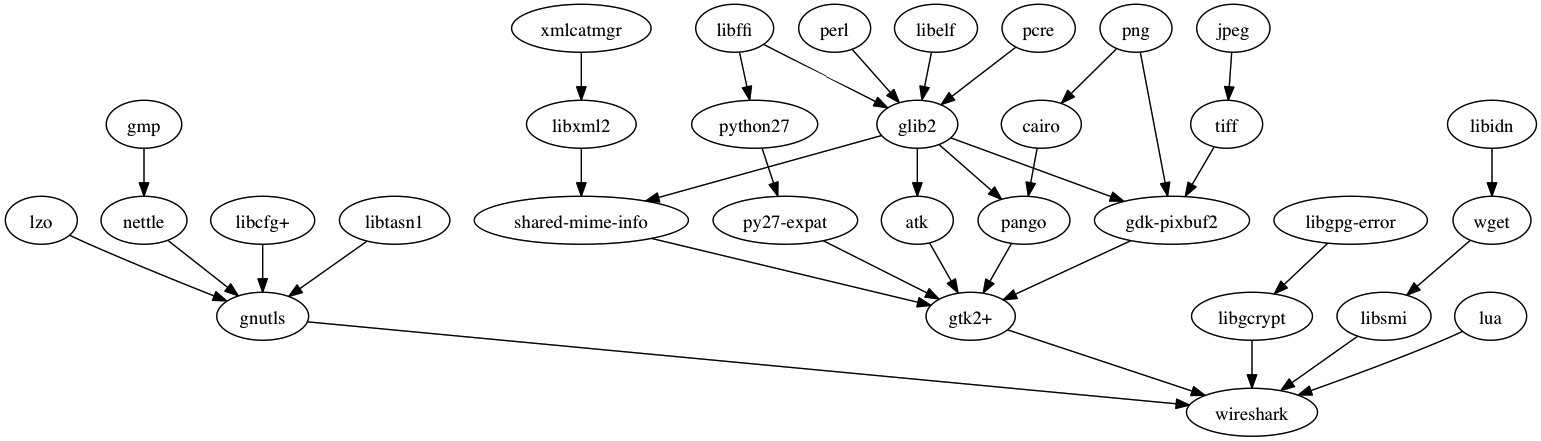
\includegraphics[width=0.95\textwidth]{05/pics/wireshark-dependencies}
		\caption[Software Dependency Tree]{Dependency graph for
			the ``Wireshark'' package, a popular network
			protocol analyzer.
			Package management systems help track such
			intricate dependencies.
			\label{fig:os-installation:wireshark}}
\end{figure}


\begin{itemize}
	\item {\bf Easy package installation.} The most obvious and
		frequent use of the package manager is to install
		software.  These tools usually allow you to only specify a
		name, and they will fetch all required files (including
		pre-requisites) from the Internet, your intranet, or a
		local storage medium and install all the files with the
		right permissions in the right places.

	\item {\bf Automatic resolution of software dependencies.}
		\index{Software!Dependency Tree of}
		Most software relies on specific libraries to be present
		on a system in order to run.  Sometimes the requirements
		are restricted to an operating system, a kernel version or
		another core system component, but more often than not a
		piece of software requires you to install other packages
		in order to be able to use it.

		These software dependencies quickly grow complex: consider
		the requirements expressed in the graph shown in Figure
		\ref{fig:os-installation:wireshark}: in order to be able to
		use a single piece of software, thirty (!) other components
		needed to be installed.  Updating any one of these could
		lead to problems further down in the graph -- and this is
		only a subgraph of the entire system's dependency tree!

		Package management systems keep track of these
		dependencies and allow you to automatically add
		pre-requisite software packages as well as prevent you
		from accidentally removing a component relied on by other
		packages.

	\item {\bf Package inventory.}  As software is installed, the
		package manager keeps track of which packages are added,
		allowing you to get a full list of all software names and
		version numbers in use on any given host.  This, in turn,
		makes it easy for you to identify any required updates, as
		package managers allow you to check whether or not newer
		versions of any given package might be available.

		Some systems even integrate security checks: by comparing
		the list of installed packages to one or more lists of publicly
		known software vulnerabilities, you can get alerted when
		an exploit affecting your hosts has been announced.  Even
		if a fix has not yet been released, this information is
		invaluable, as often you are able to take other measures
		to mitigate the risk.

	\item {\bf File inventory.}  One of the most essential properties
		of any package manager is that it tracks which files belong
		to which package, allowing you to to easily identify the
		purpose of any file or to at least lead you to more
		information about it.

	\item {\bf File integrity.}  Since the package manager already
		maintains a file inventory, it is trivial to also track
		checksums for all files that are installed -- in fact,
		most already do.  This can be used as the basis for a
		simple host-based intrusion detection system.

	\item {\bf Security.}  By downloading source
		code and compiling it on your systems, you are
		inherently trusting the sites from which you retrieve
		the code as well as the transport mechanisms by which
		you did retrieve them.  You are implicitly trusting
		the remote code repository and access restrictions on
		those systems.  That is, you win no security
		assurances unless you manually audit all code paths
		and all dependencies.  This is simply not practical.
		Using signed binaries or packages
		provided by the software project maintainers overcomes
		many of the issues here.

		(It is no coincidence that this last bullet point
		reflects the security concerns we noted in the
		previous section.)

\end{itemize}

\begin{lstlisting}[float,label=code:rpm,caption={[{\em
rpm}/{\em yum} sample commands]Example invocations of
the {\em rpm}/{\em yum} package manager to add a
package, list its files and identify the name of a
package a given file belongs to.}]
$ sudo yum install screen
Password:
Setting up Install Process
Resolving Dependencies
[...]
Updated:
  screen.x86_64 0:4.0.3-16.el6

Complete!
$ rpm -ql screen
/etc/pam.d/screen
/etc/screenrc
/usr/bin/screen
[...]
$ rpm -qf /usr/share/man/man1/screen.1.gz
screen-4.0.3-16.el6.x86_64
$ 
\end{lstlisting}


By using a package management solution, we can build a
central software inventory, which we can then map to a
host's function.  By defining conceptual roles a host
may perform, the software (and in particular what
versions of the given software) to be installed
becomes a configuration option that can easily change
at runtime.  This in turn gives us significant
advantages in our three desired key areas:
scalability, simplicity, and security.  In order to
ensure system consistency across large numbers of
hosts, we can more easily integrate binary packages
into our service inventory and deployment system
(``hosts functioning as web servers will get the {\tt
apache-2.4.3}\index{\tt apache} package installed'') and software
upgrades or patches can consistently be applied using
the same set of tools; we significantly simplify
virtually all operations that require a lookup of what
files are present on which hosts, what version of what
software is running at a given time and how to perform
upgrades with both simple or complex dependencies; by
tracking all software versions and the files the
packages contain, we can easily check for known
vulnerabilities and quickly patch the software.

\begin{lstlisting}[float,label=code:pkg_add,caption={[{\em
pkgrsc} sample commands]Example invocations of the
{\em pkgsrc} package manager and related tools to
visualize package dependencies.  Figure
\ref{fig:os-installation:wireshark} was created using
these commands.}]
$ pkg_add wireshark pkgdepgraph graphviz
$ pkg_info -n wireshark
Information for wireshark-1.8.3:

Requires:
gtk2+>=2.24.12nb3
glib2>=2.32.4nb1
pcre>=8.30nb1
lua>=5.1.4nb1
libsmi>=0.4.5nb1
libgcrypt>=1.4.6nb2
gnutls>=3.0.17

$ pkgdepgraph -S ++wireshark | \
        dot -Tpng > wireshark-dependencies.png
\end{lstlisting}

None of this is possible without the use of a package
management system, but these benefits come with a
price: the packaging system must be used consistently
for {\em all} software.  The act of adding a piece of
software outside this mechanism opens up the
possibility for a broken dependency graph and often
triggers future ``forced'' installations of packages
(i.e. overriding warnings about unmet dependencies,
since the packaging system has no way of knowing what
we installed outside of its catalog) and finally the
loss of a coherent inventory.

Hence it is crucial to be consistent and perform the
at times tedious and frustrating work of
(re-)packaging software in the format that best
integrates with your deployment and management
solutions.  This gets increasingly difficult, as
individual programming languages nowadays come with
multiple (!) language-specific package managers of
their own (see Figure
\ref{fig:software-installation:pip-bower}), as each
language develops its own ecosystem of software
components that their creators cannot provide for {\em
all} possible package managers.

Finally, need to make sure to {\em also} build
packages for all of the software that we do not
retrieve from other sources, for our own software.
That is, when we build software, we have to package it
up and integrate it into our software inventory.  As
we will see in Chapter
\ref{chap:building-scalable-tools}, system
administrators write a {\em lot} of software: we write
small and simple tools just as we write large and
complex infrastructure components; all of these need
to be installed, updated, maintained.  Our own
software is no different from software provided by
others, and so we owe it to ourselves to package it
properly as well.

\begin{figure}[t]
	\centering
	\subfloat[What's pip?]{\label{fig:software-installation:pip}
				\raisebox{.5em}{
					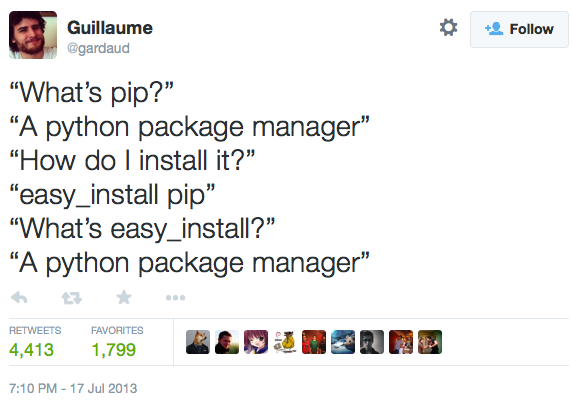
\includegraphics[width=.45\textwidth]{05/pics/pip}}}
	\hspace{1em}
	\subfloat[What is bower?]{\label{fig:software-installation:bower}
				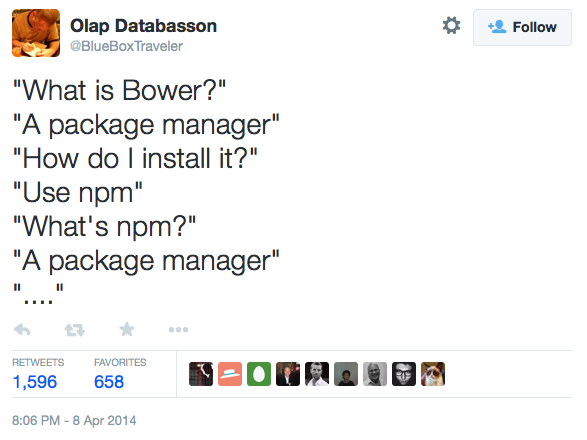
\includegraphics[width=.45\textwidth]{05/pics/bower}}
	\caption{Screengrabs of tweets illustrating the
		circular dependencies of language-specific package
		managers ca. 2014.\label{fig:software-installation:pip-bower}}
\end{figure}



\subsection{Inherent Security Risks}
\label{software-installation:package-management:security-risks}

When we install any software, no matter which method
we use, we are exposing our system to the risk of a
software Trojan, the accidental installation of a
backdoor, a piece of malware\index{malware}.  In an
ideal world, we would verify the integrity of the
software and review what it does, what resources it
utilizes and what information it accesses, receives or
sends.  Unfortunately, doing this for all the software
we download and install is simply not possible, and so
we routinely fetch code from the Internet, compile it
and install the resulting executable.

When we perform these steps, we trust that the code we
are about to install is not malicious because... well,
we just assume that if it was, surely somebody else
would have noticed.  And besides, the website we
downloaded it from looked rather nice, too.  But
suppose that even if we knew that the software we want
to download is not malicious, how do we know that we
are in fact getting it from the website that we {\em
think} it's coming from?

In theory, we can ensure the integrity of the download
by only using secure transport mechanisms (over TLS,
for example) and by verifying a checksum published on
the website in question after the download.  In
practice, doing this work does, once again, not scale:
there simply is too much software released without any
such information.  Fortunately for us, a good package
manager can help in this area, too!

The build process for most software package management
systems ultimately requires a human to decide what
sources to build the software from, and so we are,
when using the resulting binary packages, shifting our
trust from the software provider to the software {\em
package} provider.  Often, these two are the same
person or within the same organizations, but in some
cases, the party providing the package is not the
owner or developer of the software in question.  Just
think of the thousands of RPM or Debian packages
provided by RedHat\index{RedHat} or
Ubuntu\index{Ubuntu}, or the software re-packaged by
the FreeBSD {\em ports} or NetBSD {\em pkgsrc}
systems.

What's more, all software package management systems
need to be able to not only install files, but to run
certain commands required for the proper installation
and configuration of the software in question.  To
this end, they provide the capability for a given
package to execute an arbitrary shell script provided
in the package, with the privileges of the invoking
using -- commonly the superuser.

In other words, it is important to understand that any
time we use a package manager to retrieve and install
software for us from the Internet, we effectively let
it fetch and execute unknown code on our systems.
That is, not only do we trust the package manager
locally -- as well as the software author(s) -- we {\em
also} (and implicitly) trust the people who run and
maintain the package repositories.  These repositories
are managed by system administrators like ourselves --
mere mortals, as highly as we may think of ourselves
-- and every once in a while mistakes are made, and
accounts are compromised, putting at risk users of the
software hosted there worldwide.\footnote{In 2003, the
\gls{gnu} Project's primary FTP server was
compromised.  The possible impact of this is
staggering, given the number of projects that are
relying on the software provided there.  During the
clean-up after the event, every software package had
to painstakingly be verified against known good
checksums, which in many cases were missing and had to
be first identified from other sources.}

Then what is the solution to this problem?  Well,
unfortunately there simply isn't a solution.  We can
build more and more complex systems that provide
better authenticity and better assurance of integrity,
but at the end of the day, we still have to place
trust into systems built and maintained by others.
Ken Thompson's \index[names]{Thompson, Ken} Turing award
acceptance speech ``Reflections on Trusting
Trust''\cite{thompson:trust} cannot remain unmentioned
in this context.  If you are not familiar with this
short paper, look it up on the Internet -- it's
Zen-like moral will change how you regard system
security.

Despite our having to trust so many components outside
our control, and despite the fact that we cannot
eliminate all risks involved, it is important that we
are aware of them.  A good package manager will
provide you with reasonable options to automatically
determine updates from trusted sources and optionally
even apply them.  This requires a significant reliance
on the trustworthiness of the package manager, and
only when we understand the risks can we make informed
decisions.  Perhaps we'll be even a little bit more
careful and observant about how and where our package
management system retrieves its data from or what
other resources we allow it to use.

\section{Managing Software Updates and Patches}
\label{software-installation:managing-updates}

Despite the security concerns, we have praised package
management systems in the previous section as a
reasonable solution to many problems.  Unfortunately,
updating software remains fundamentally difficult and
carries significant risk.  Every time you change a
system component, you are introducing new elements
into your environment and the probability of
unexpected side-effects increases the larger the
change set is.

``If it ain't broke, don't fix it.''\index[names]{Lance, Bert}
has become many a system administrator's mantra,
meaning that unless you have a {\em very} good reason
to change something on a system that is currently
running and not experiencing any problems, you
shouldn't do so.  This simple lesson needs to be
learned over and over again by every system
administrator, and it appears it cannot be learned
without a modicum of self-inflicted
pain.\footnote{Part of this lesson is to understand
that a security problem may very well require us to
judge the software as ``broken'' as any functional bug
or a decrease in usability.}

At the same time, we require agility and high
confidence in our ability to apply significant
changes, to perform package and OS upgrades on a
regular basis.  These conflicting goals -- stability
and agility -- will be part of our discussion of
managing system services in Chapter
\ref{chap:services}. \\

The benefit of a package manager's dependency
resolution has the often undesired result that a
number of pre-requisites or dependencies further down
the graph need to also be updated when a simple
software change to a single package was desired.
Therefore, {\em all} software updates need to be
treated with great care.

The conservative stance hence remains to leave your
system running as is instead of chasing every new
software release, every minor OS update or even to not
bother applying patches if a software vulnerability
appears to not directly impact you.  Unfortunately,
this will make it the more likely that {\em when} an
upgrade finally is required, it will pull with it a
significant number of other changes.  There is no
one-size-fits-all solution to this problem; every
system administrator has to make these decisions for
themselves according to their specific environment.
Until experience allows you to confidently make this
call, it is probably wise to consider any known
security issue to at least warrant very careful
analysis of the possible impact.  \\

When evaluating the need to upgrade a piece of software, it is important
to consider a number of factors:

\begin{itemize}

	\item {\bf Be aware of software updates.}  In order to be able to
		judge whether or not your software needs to be updated,
		you first need to know when new releases are available and
		what features they might include.  Most operating systems
		provide a channel with regular information about release
		updates -- make sure to subscribe to these.  Likewise, you
		probably should track the development process of all your
		major infrastructure components or important products
		(inside or outside your organization).

	\item {\bf Track security updates and announcements.}  Your
		software provider (OS or otherwise) is likely to have a
		mailing list or other information channel dedicated to
		security updates for their software.  You should follow
		these and make sure to evaluate all updates with
		particular attention.

		In addition, you should subscribe to some of the
		mailing lists where vendor-neutral public security
		announcements are posted.\footnote{The ``Bugtraq'' and ``Full
		Disclosure'' mailing lists are two examples.  Searching
		the Internet for these terms should quickly yield the
		right results.} It is not uncommon to first hear about a
		vulnerability for one piece of software here, only to
		find out later on that it also applies to other variations
		you might be running.

	\item {\bf Consider privilege escalation possibilities.}
		Sometimes there are vulnerabilities that do not seem to
		apply to your specific environment, but that can become
		severe when combined with another low-risk vulnerability.
		Make sure to consider all aspects of how your systems
		might be accessed or used when assessing the severity of
		any known vulnerability in the software that you run.
		(We will cover this in more detail in chapter
		\ref{chap:security}.)

	\item {\bf Consider the impact of updating {\em shared
		libraries}.}  The benefit of using shared libraries (no
		need to update all software components using these
		libraries) can become a drawback when a widely used
		library needs to be updated.  As much as software
		providers attempt to provide backwards compatibility,
		sometimes it is (intentionally or coincidentally) broken.
		Software using this library may suddenly start to behave
		erratic or completely stop to function.  Other upgrades
		may even be known to break certain dependent systems.

		It is important to test your software upgrades to ensure
		at least the most basic compatibility is preserved, but
		since it is impossible to exercise all possible code
		paths, you should also weigh the possible impact the
		upgrade may have against the benefits provided by the
		upgrade.

	\item {\bf Consider the impact of updating
		{\em static libraries}.}  This may generally be
		thought of as a less frequent use case, but some
		components may be provided to you or installed on your
		systems using statically linked libraries.  However,
		in the last couple of years (between 2012 and 2017),
		we have seen a tremendous influx of the use of the
		``Go'' programming language (which produces statically
		linked binaries) as well as -- effectively -- by way
		of containers. Here, the update of a package providing
		the library has no effect on the applications using
		this library or the software running inside a
		container -- in order for the change to take effect,
		these applications would need to be re-linked, the
		containers to be restarted.

	\item {\bf Restart applications after the software update.}  In
		order to ensure that all updates have actually taken
		effect, it is usually necessary to restart at least the
		application(s) in question, if not reboot the entire
		system (such as in the case of a kernel or core library
		upgrade).  This implies a service disruption of anywhere
		from a few seconds to several minutes or even longer.
		\footnote{This brings with it the problem of system-wide atomicity
		of software upgrades: it is generally not advised to run a
		given service using different versions of their software
		across multiple systems.  Upgrading all hosts at the same
		time, however, carries the risk of breaking functionality
		(not to mention overall service down time).  Deploying
		such upgrades in a controlled manner across large numbers
		of systems is beyond the scope of this chapter; in fact,
		it easily warrants an entire book by itself.  We'll scratch
		that surface in Chapter \ref{chap:services}.}

	\item {\bf Verify the integrity of your updates.}  When you
		receive software updates, it is important to verify that
		they are in fact updates provided by your provider.  Most
		software distributors cryptographically sign all their releases
		(including software patches), making it easy for you to
		check the integrity of the update.

		Similarly, and depending on the scale of your
		organization, your own infrastructure tools used to roll
		out updates should automatically check all software
		updates in this manner.

	\item {\bf Create your own patches.}  At times, you will find
		yourself in a situation where you need to update a piece
		of software, but the provider has not (yet) released a
		patch.  In some cases you may be able to avoid the problem
		at hand by removing or restricting certain functionality;
		other times, you may be able to fix the problem yourself.

		If you are able to create a patch for a given
		vulnerability, to add a desired feature, or to merge
		another update from a different source, please consider
		contributing it back to both the original software
		creators, as well as to the general public community
		around the software.  Others will surely appreciate this
		help!
\end{itemize}

As you can tell, the above considerations suggest that
determining when, or even {\em if}, you can upgrade
software is far from easy and requires an intimate
understanding of all the details of the running
system.  Even though you can automate the updates of
your software across even hundreds of thousands of
hosts, you cannot automate making the decision to
upgrade.  As a system administrator, this burden is on
you.


\section{Conclusions}
\label{software-installation:conclusions}

In this chapter we have taken a closer look at how
software is installed on a system.  As we reviewed the
boot process, we distinguished between different types
of software, and identified a few distinct categories:
firmware and device drivers, the kernel managing all
hardware and interfacing with the drivers, a number of
core system components such as essential system tools
and libraries, basic applications and utilities
required to make the system usable, and finally
entirely optional add-on applications.  The
distinction between these categories has proven to be
difficult to make, which is why we have further
divided types of software by their place in the file
system hierarchy into the four categories of being
``shareable'', ``unshareable'', ``static'' or
``variable''.

We have looked at the steps required to install an
operating system and discussed the need for a package
management solution to keep track of all files on the
system, as well as the implications of any required
software upgrades.  A package management system, a
requirement for addressing a number of problems when
maintaining large systems with many pieces of software
installed, does not come without its price, however.
As we have stressed, it is important to make {\em
consistent} use of the chosen package manager, but
this has become increasingly difficult: on the one
hand, configuration management tools are able to
manipulate files ``owned'' by the package management
system; on the other, not all software you need to
install is available in the given format.

Building your own packages from sources is laborsome.
What's more, it can be frustrating, as you are
duplicating work already done by others to some
extent.  This holds especially true with respect to
many programming languages and the many smaller
components or modules available for them.  Almost
every modern programming language nowadays includes
its own preferred way of installing language modules
(including the search for and retrieval of the
``right'' version from an online repository).  There
is an old joke in which people lamenting the existence
of too many competing standards get together to create
the one true solution only to end up with just one
more competing standard with limited adoption.  We can
see this holding painfully true when we look at how
different language developers have all solved the same
set of problems (slightly) differently:

Perl has used its {\tt CPAN}\index{CPAN}
infrastructure for decades; Python uses its {\tt
pip}\index{pip} installer; software written in the
Ruby language is often provided as so-called
``gems''\index{RubyGems}; Node.js uses its own package
manager, called {\tt npm}\index{npm}; PHP applications
or extensions are distributed using the {\tt PEAR}
framework and so on.  Each of these tools allows a
package to easily express its requirements on other
language components, but none of these integrates
really flawlessly with other, non language-specific
package managers. (See again Figure
\ref{fig:software-installation:pip-bower}  People
using the RedHat Package Manager (RPM)\index{RPM}, for
example, end up having to re-packaging these modules
or risk breaking their package consistency model.

Others choose to let yet another tool control the
deployment of their software: more than once did we
have to note that defining what software packages or
versions need to be installed on a system is not a
one-time act performed at OS installation time.
Instead, controlling what software is added or
removed, updated, activated or in other ways
manipulated is part of an ongoing process and easily
becomes part of the larger topic of Configuration
Management\index{Configuration Management}.  In fact,
many configuration management solutions -- systems
that apply software configuration changes at runtime
-- include functionality to either require software
packages to be present or are even able to install
them as needed.  We will revisit some of these aspects
in coming chapters.

\vfill
\pagebreak

\chapter*{Problems and Exercises}
\addcontentsline{toc}{chapter}{Problems and Exercises}
\section*{Problems}
\addcontentsline{toc}{section}{Problems}

\begin{enumerate}
\item
Observe the boot process of various systems in your environment.  What
kind of firmware, boot loaders and system software is involved?  Do you
have different boot options leading to a running system with a different
kernel or support for different features?

\item
Review the manual pages (and/or other documentation) of the boot loader(s)
used in your environment.  How hard or easy is it to modify the boot
process?

\item
Review the {\tt hier(7)} manual page on your preferred Unix version.
Identify which components are specifically designated for single- and
which for multi-user operations of the system.  Does the manual page hint
at a separation between shareable and unshareable, static and variable
data?  Compare to two other Unix systems.

\item
Cross-reference the examples in Table
\ref{table:software-installation:shareable-variable} to your system's
manual page or build your own matrix to help yourself identify how the
traditional Unix file system hierarchy applies this model.  Identify three
directories for each combination.

\item
Considering file system and OS implications, identify the hardware and
software requirements for each of the following systems.  Research and
compare common performance requirements and real world use cases to your
suggested solutions.

\begin{enumerate}
\item
a number of web servers, able to efficiently serve tens of GB of small
static files

\item
a number of web servers, able to efficiently serve dynamic content (using
any of the various popular languages and frameworks, such as PHP, Ruby on
Rails, Scala, ...)

\item
a central server hosting a source code repository (very large amounts of
small files with frequent changes, requiring lots of fast I/O and high
data redundancy requirements)

\item
a general purpose workstation / desktop system
\end{enumerate}

\item
\label{prob:software-installation:os-installation}
Perform a basic OS installation of your Unix flavor of choice on a hard
drive (or in an emulator on a disk image).  Note the default values chosen
by the OS, such as partitioning schema, file system choice, number of
packages installed, services enabled and user accounts created.  What type
of system is the OS optimized for?  Do the default installation choices
make this OS more or less suitable for any specific use case?  Consider
the use of the system as a desktop system, a scientific work station, and
a generic Internet facing server.

\item
\label{prob:software-installation:os-installation:manual}
Perform a basic OS installation of your Unix flavor of choice on a hard
drive (or in an emulator on a disk image) without using the OS provided
installer.  That is, perform the steps needed to install an OS on a disk:
partition the hard drive, create a new file system, install a boot loader,
extract the basic OS sets or install the basic OS packages onto the new
disk, add user accounts as needed, enable system services as needed, etc.

\item
Identify the package manager running on your systems and make yourself
familiar with it.

\begin{enumerate}
\item
List all packages installed on your system with version numbers.  Identify
packages that have other packages depend on them as well as ``leaf'' packages
(those without any other package depending on them).  Which package has
the most dependencies, which one is the most depended-upon?

\item
What are the commands to install a piece of software?  To delete a
package?  To upgrade a package?  To downgrade a package?

\item
What are the commands to list the files installed by a given package?
Given a file name, how do you identify what package it belongs to?
\end{enumerate}

\item
\label{prob:software-installation:pkg-vs-manual}
Create virtual OS instances of a few different operating systems, such as
NetBSD, FreeBSD, different Linux versions, and Solaris.

\begin{enumerate}
\item
Compare their default installations.  What kind of packages are installed
on each system?  What kind of services are enabled by default?

\item
Using their default package management system, install the latest versions
of the following software: gcc, perl, python, gnupg, screen, sudo.  How
does the software installation procedure differ?  How can you upgrade or
remove the software?

\item
Using the {\em pkgsrc} cross platform package manager, again install the
same software into a different prefix.  How does the software installation
procedure differ from the native package manager?  How does it differ
across the different systems?  How can you upgrade or remove the software?

\item
Download the source for the same software from their respective
repositories and install it a third time, this time using no package
manager at all.  That is, follow the installation instructions found in
the software package, possibly using the common {\tt ./configure; make;
sudo make install} sequence.  How does the software installation
procedure differ across the various systems?  How can you upgrade or
remove the software?
\end{enumerate}

\item
\label{prob:software-installation:build-a-package}
Identify a piece of software you commonly use, but that is not packaged
for your primary platform.  Create a package for it, then contribute your
changes back to the original author(s) of the software.

\item
All package management systems have certain drawbacks.  Eventually, a lot
of people conclude that the only solution to their problems is to write
their own.  Regardless of the correctness of this conclusion, let us
assume you are in this position.  How would you design a package manager?
Write down the hard requirements it needs to meet, the challenges it needs
to overcome, and identify any optional features.

\item
Review a recently identified security vulnerability in a popular piece of
software.  How were the patches or updates made available?  Can you verify
their authenticity and integrity?

\end{enumerate}

\pagebreak

\bibliographystyle{plainnat}
\begin{thebibliography}{99}

\bibitem{software:silberschatz}Abram Silberschatz, Greg Gagne, Peter B.
Galvin {\em Operating System Concepts}, John Wiley \& Sons, 2011

\bibitem{fhs}Daniel Quinlan, Paul Russell, Christopher Yeoh (Editors) {\em
Filesystem Hierarchy Standard}, Filesystem Hierarchy Standard Group
{\url http://www.pathname.com/fhs/pub/fhs-2.3.html} (visited November 13,
2012)

\bibitem{nemeth:unix-handbook}Evi Nemeth, Garth Snyder, Trent R. Hein, Ben
Whaley {\em UNIX and Linux System Administration Handbook}, 4th Edition,
Prentice Hall, 2010

\bibitem{thompson:trust}Ken Thompson {\em Reflections on Trusting Trust},
Communication of the ACM, Vol. 27, No. 8, August 1984, Association for
Computing Machinery, Inc.; also available on the Internet at
{\url http://cm.bell-labs.com/who/ken/trust.html}
(visited December 5th, 2012)

\end{thebibliography}
